\documentclass[12pt]{book}
\usepackage[width=4.375in, height=7.0in, top=1.0in, papersize={5.5in,8.5in}]{geometry}
\usepackage[dvips]{graphicx}
\usepackage{amsmath}
\usepackage{amssymb}
\usepackage{tipa}
%\usepackage{txfonts}
\usepackage{textcomp}
%\usepackage{amsthm}
%\usepackage{array}
%\usepackage{xy}
\usepackage{fancyhdr}
\usepackage{listings}
\lstset{breaklines=true}
\usepackage[titletoc]{appendix}

\pagestyle{fancy}
\renewcommand{\chaptermark}[1]{\markboth{#1}{}}
\renewcommand{\sectionmark}[1]{\markright{\thesection\ #1}}
\fancyhf{}
\fancyhead[LE,RO]{\bfseries\thepage}
\fancyhead[LO]{\bfseries\rightmark}
\fancyhead[RE]{\bfseries\leftmark}
\renewcommand{\headrulewidth}{0.5pt}
\renewcommand{\footrulewidth}{0pt}
\addtolength{\headheight}{0.5pt}
\setlength{\footskip}{0in}
\renewcommand{\footruleskip}{0pt}
\fancypagestyle{plain}{%
\fancyhead{}
\renewcommand{\headrulewidth}{0pt}
}
%
%\parindent 0in
\parskip 0.05in
%
\begin{document}
\frontmatter
\pagestyle{empty}
%\pagenumbering{}
% Set book title
\title{\textbf{A course on Quality of Service (QoS)}}
% Include Author name and Copyright holder name
\author{Jaume Barcelo}
% 1st page for the Title
%-------------------------------------------------------------------------------
\maketitle
%
\pagestyle{fancy}
%
\tableofcontents
%
\mainmatter
%
\chapter{About the course}

\section{Course Data}

Code: 21738

Course name: ``Protocols de qualitat de servei en xarxes''

Teacher: Jaume Barcelo

Credits: 4

Year: 3rd year

Trimester: Spring

\section{Introduction}
This is a course on Quality of Service in data networks, which is usually abbreviated as QoS.
QoS is about discriminating traffic.
It is about favouring some data packets at the expense of others.
The name can be misleading, as one might think that all packets are benefited from the implementation of QoS.
This is not the case.

A good parallelism to understand QoS is road traffic.
There are some vehicles (typically police, ambulance and firefighters) that receive priority over the others. 
This is not perceived as something negative, as this vehicles incur in tasks that are more important or urgent than the average vehicle.

This parallelism is very illustrative to convey the idea, that QoS does not make the road wider, it simply prioritizes some traffic.

At some point, networks engineers may face the dilemma of investing their efforts and money in either implementing QoS (prioritizing traffic) or increasing the available bandwidth (making the road wider).
The latter option has the advantage that it benefits all the traffic of the network.
Ideally, if the bandwidth is sufficiently over-provisioned, the packets never have to wait in the routers queues.
In the road analogy, if the roads are wide enough, there are never traffic jams.

Unfortunately, making the roads wider or the networks faster does not always solve the problem.
As the users perceive that there is plenty of bandwidth available, they might decide to put it a better use by downloading collections of movies that they will never have time to see.
There is nothing wrong with downloading collections of movies, but the sheer volumes of data may fill up the queues and introduce unacceptable delay and jitter in VoIP calls.

And why is this a problem? Well, at some point network engineers that deploying separate networks for each service represented too much work (and money).
From an engineering and economic point of view, it is much more advantageous to offer the different services on a single network.
It is common nowadays that telephony, video-conference, web, remote backup and file sharing services share the same network.
The term to refer to these networks that support various services is ``converged networks''.
The only problem is that the different services have totally different requirements with regards to required bandwidth and delay.

The service that consume a large amount of bandwidth and do not have strict delay requirements can easily create a ``traffic jam'' that prevents the offering of services with low delay requirements that consume very little amount of bandwidth.
Obviously, it is still possible to offer the two kinds of service simultaneously if we implement QoS mechanisms that prioritizes the low delay traffic.

QoS is a controversial topic.
Net neutrality, which is related to QoS is even more controversial \cite{bachula2006}.
Nevertheless, QoS (or ``bandwidth management'') has been used by ISPs in practice \cite{cooper2011bum}.
We will try to cover the subject from a neutral point of view and you, equipped with the knowledge of the course, will take your own decision about the usefulness of QoS.

The course is divided in three conceptually different parts: lectures, seminars and lab assignments.
In lectures I will introduce you to the nuts and bolts of QoS.
In the seminars, we will review the concepts of queueing theory covered in previous courses, and extend them to consider different traffic classes.
In the lab assignments you will implement some QoS tools and, when possible, validate them with the methods studied in the seminars.

\section{Syllabus}
\begin{itemize}
  \item Lectures
  \begin{enumerate}
    \item Introduction to QoS
    \item QoS Requirements
    \item QoS Service Level Agreements
    \item QoS Mechanics
    \item QoS Architectures
    \item Deploying Diffserv
    \item Capacity Admission Control
    \item SLA and Network Monitoring
    \item Core Capacity and Traffic Engineering
  \end{enumerate}
  \item Seminars
  \begin{enumerate}
    \item Review of basic concepts. Exponential distribution. Poisson Traffic. Little's Theorem. PASTA theorem.
    \item Delay in a network interface with Poisson arrivals, a single (finite) buffer and exponential transmission time.
    \item Delay in a network interface with Poisson arrivals, two traffic classes and exponential transmission time. Preemptive priority and non-preemptive priority.
    \item Delay in a network interface with a general transmission time. Priority queueing in a network with a general transmission time.
  \end{enumerate}
\item Lab Assignments
  \begin{enumerate}
    \item Program a UDP Poisson traffic generator and a traffic sink capable of computing delay (min/avg/max). Packet drop should also be measured.
    \item Program a packet buffer. It should support both exponential and deterministic transmission time. The buffer size is taken as a parameter and it may be infinite.
    \item Program a buffer that implements priority queueing. It should support both exponential and deterministic transmission time. The buffer size is taken as a parameter and it may be infinite.
    \item Implement a QoS tool of your choice: policer, token bucket, leaky bucket.
    \item Combine the different QoS elements that you and your classmates have programmed in a QoS enabled network. Invent an scenario, describe the requirements and explain how your solution addresses such requirements.
  \end{enumerate}
\end{itemize}

\section{Bibliography}

The lecture closely follow the book:

John Evans, Clarence Filsfils ``Deploying IP and MPLS QoS for Multiservice Networks''.

\section{Evaluation Criteria}

The grading is distributed as follows:
\begin{itemize}
\item Lectures continuous assessment, 10\%
\item Seminars continuous assessment, 10\%
\item Blackboard problem solving, 10\%
\item Lab assignments, 10\%
\item Individual continuous assessment quiz, 10\%
\item Final exam, 50\% (Possibility of re-take exam)
\end{itemize}

It is necessary to obtain a decent mark (4 out of 10 or 20 out of 50) in all the different evaluation aspects.
To pass the course, 50 out of the total 100 points need to be obtained.

\section{Survival guide}

\subsection{How to pass the course}

Statistically speaking, you will pass the course if you do all the following:
\begin{itemize}
\item Attend lectures, participate and ask questions.
\item Attend seminars, try to solve the problems on your own and discuss them in small groups.
\item Volunteer to solve problems on the blackboard.
\item Attend labs and use lab time to solve the lab assignments.
\item Participate in the planning and coding of the labs assignments. Read carefully the code of other team members and make sure you understand it and can explain it to others.
\item Study for the continuous assessment quiz, as it is a warming up exercise to face the final exams with success guarantees.
\end{itemize}

\subsection{Continuous Assessment}
In this course we implement continuous assessment.
This means that if you work hard from day zero, the course will be pain-free.

Continuous assessment includes multiple-choice quizzes in lectures and seminars.
You also have to write reports in labs (one for each group).
The source code and the report for the labs is submitted via moodle.
Remember to write always your name and NIA in all the material you hand in or upload to moodle. 
You also have to include you name and NIA in all the source code files you send me.

There is not a template for the report.
I recommend describing key design and implementation aspects, clarifying possible deviations or improvements on the initial assignment, and including examples.
The example should include the input commands as well as the output results.
The report and the code will be submitted at the end of the class via moodle.
At the beginning of the next class, you will have to demonstrate that your programs actually work.

\subsection{Collaboration Policy}
You are encouraged to collaborate with other students in the resolution of problems and assignments.
However, you should firs try to solve it on your own.
Then, you can discuss your solution with others and work together to find a better solution.
Finally, you must ensure that you can solve the problem or assignment alone.

In the labs assignments you will work in teams of three people.
Unless when explicit permission is given to re-use code, each team has to write their own code.

\subsection{Formula Sheet}
This course is not about memorizing equations.
It is about understanding them.
For this reason, you are allowed to use a \emph{formula sheet} in individual tests as long as it fulfills the following requirements:
\begin{itemize}
\item It is a single page (one side).
\item It is handwritten. Your own handwriting.
\item It is delivered together with your answers when the test is finished.
\end{itemize}

\subsection{Questions and doubts}
I like to receive questions and comments.
Normally, the best moment to express a doubt is during the class, as it is likely that many people in the class share the same doubt.
If you feel that you have a question that needs to be discussed privately, we can discuss it right after the class.

\subsection{Continuous feedback}
At the end of the class, I will ask you to anonymously provide some feedback on the course. 
In particular, I always want to know:
\begin{itemize}
\item What is the most interesting thing we have seen in class.
\item What is the most confusing thing in the class.
\item Any other comment you may want to add.

In my previous experience, this information has proven to be invaluable in improving the course, detecting problems at an early stage, and adapting the course to the expectations of the students.

In labs, I will ask each group to hand in a short (few paragraphs) description of the work carried out in class, and the members of the group that have attended the class.
Note that this is different from the lab report, which is the one that it is actually graded.
\end{itemize}

\subsection{How to make you teacher happy}

Avoid speaking while I am talking.
It is not that you cannot talk in class.
You can talk as much as you want when I am silent.
I will make plenty of breaks in which I will ask you to discuss a question with your classmates.
You can also take advantage of the moments in which I erase the blackboard or just scratch my head while staring.
As long as I am not talking, you can talk with your classmates as much as you want.
Obviously, questions are welcome at any time.

\chapter{QoS metrics}
\label{cha:quality_metrics}

If you go to the postal office to submit a packet, you will be offered different options.
In addition to the regular service, it is possible that an urgent service exists.
Probably there is also the possibility sending the packet as certified mail, and some option for delivery notification.
It is likely that there are also special services for packets that are voluminous or heavy.

QoS-enabled packet switched networks also offer different kinds of services for data packet delivery.
In this chapter, we will review the different metrics that are relevant for data networks.
This metrics can be used to establish \emph{service level agreements} (SLAs) which are contracts specifying the QoS expected from a network.
These contracts should also specify how the metrics are actually measured.

As an example, if a network guarantees a delay below 100 ms, it should be specified whether this makes reference to the maximum, the average delay or the 95\% percentile.
The measures will also differ depending whether 5 minutes averages or 1 hour averages are considered.
This makes the specification of SLAs tricky.

\section{Delay}

Delay is the time that it is required to traverse the network from the entry point to the exit point.
Delay is normally considered for real-time services such as voice over IP (VoIP).
The total end-to-end delay is simply the sum of the delay suffered in each of the hops in the data network.
As an example, \ref{fig:four_hops} shows a network with four hops.

\begin{figure}[h]
\centering
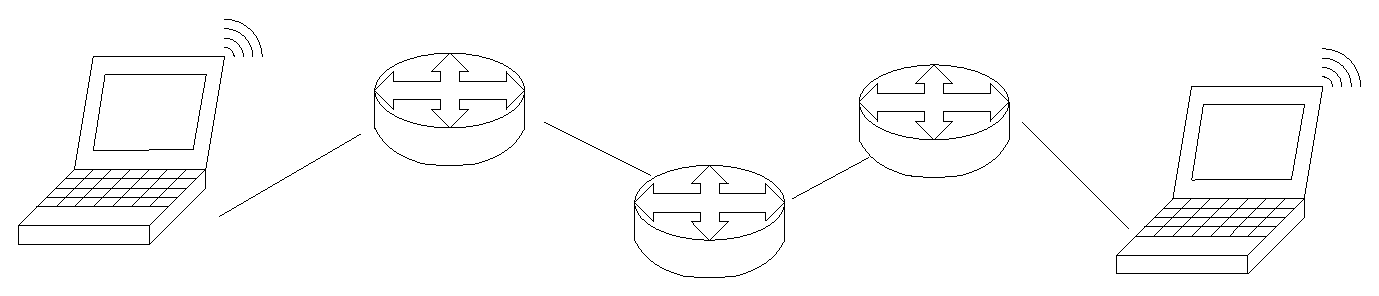
\includegraphics[width=\linewidth]{figures/four_hops.eps}
\caption{A network with two terminals, three routers and four hops.}
\label{fig:four_hops}
\end{figure}

In each hop, there are four different contributions to delay:
\begin{enumerate}
\item Processing: The time required for the router or switching device to put the packet on the outgoing interface queue.
Very short.
\item Queueing: Waiting time on the outgoing interface queue.
Very short if the queue is empty.
\item Transmission: The time required to put the packet on the transmission medium. It is a function of the packet length and transmission rate.
Short in high-speed transmission media.
\item Propagation: The time that it takes for the packet to travel the distance from the hop source to the hop destination.
Short time over short distances. 
And very long when it involves a trip to a geostationary satellite.
\end{enumerate}

\section{Jitter}
Jitter is the variation of delay.
This aspect is specially relevant for real-time and streaming applications.
These applications expect the packets to arrive regularly in time.
As an example, if the encoder application takes a voice stream and splits it into 20 ms chunks that are encoded and sent as packets, the receiver application will expect to receive one packet every 20 ms to reconstruct the voice stream.

If packets are sent every 20 ms but each of them requires a different time to traverse the network, the separation between packets will no longer be 20 ms at the receiving end.
Applications sensitive to jitter use a de-jittering buffer that holds some packets and feeds the decoder at regular intervals.
The packets that suffered a short delay in the network will wait for a longer time in the de-jitter buffer and the packets that suffered a longer delay in the network stay in the buffer for a shorter time.
With this technique, jitter is effectively suppressed at the expense of increasing delay, as shown in figure \ref{fig:dejitter}.

\begin{figure}[h]
\centering
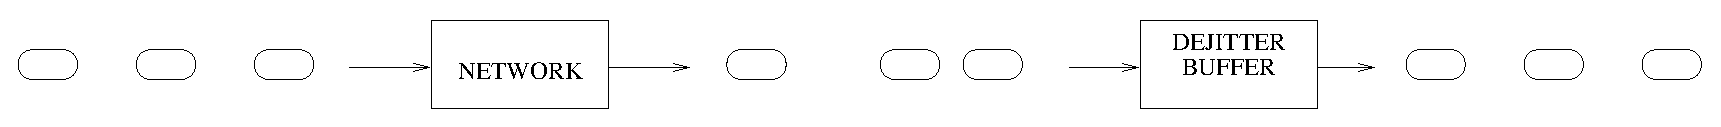
\includegraphics[width=\linewidth]{figures/dejitter.eps}
\caption{The dejitter buffer removes jitter at the expense of adding delay.}
\label{fig:dejitter}
\end{figure}

The de-jitter buffer size in terms of time and packets (or bytes) need to be carefully tuned, to prevent both packet overflow and underflow.
Buffer overflow happens when the buffer is full and cannot accommodate an arriving packet.
Buffer underflow occurs when the decoder asks for a packet and the buffer is empty.

\section{Round Trip Delay}

The round trip delay is the measure of delay used for elastic and interactive applications.
It is the time required for a packet from source to destination and then back to the source again.
You can easily find the round trip delay from your host using the ping command.

\begin{lstlisting}
$ ping www.happyforecast.com
PING happyforecast.com (184.107.100.65) 56(84) bytes of data.
64 bytes from s106.panelboxmanager.com (184.107.100.65): icmp_req=1 ttl=48 time=122 ms
64 bytes from s106.panelboxmanager.com (184.107.100.65): icmp_req=2 ttl=48 time=121 ms
64 bytes from s106.panelboxmanager.com (184.107.100.65): icmp_req=3 ttl=48 time=122 ms
64 bytes from s106.panelboxmanager.com (184.107.100.65): icmp_req=4 ttl=48 time=122 ms
64 bytes from s106.panelboxmanager.com (184.107.100.65): icmp_req=5 ttl=48 time=122 ms
64 bytes from s106.panelboxmanager.com (184.107.100.65): icmp_req=6 ttl=48 time=121 ms
^C
--- happyforecast.com ping statistics ---
6 packets transmitted, 6 received, 0% packet loss, time 5004ms
rtt min/avg/max/mdev = 121.864/122.066/122.181/0.230 ms
\end{lstlisting}

An interactive application (such as web browsing) requires a few round trip delays to complete the dialogue between the client and the server.
Furthermore, the round trip delay also limits how fast the Transfer Control Protocol (TCP) congestion window can grow.
The congestion window grows upon the reception of TCP acknowledgements.
If it takes long for the TCP acks to arrive, the congestion window grows slowly.

In fact, it becomes difficult to take fully advantage of connections with a high \mbox{throughput x delay} product.
These are known as ``long fat pipes'' or ``long fat networks'' (which is shortened as LFN and sometimes pronounced elephant), as explained in RFC 1072 \cite{rfc1072}.

\section{Packet Loss}

The networks may loose some of the packets being sent.
Packet loss has different sources:
\begin{itemize}
\item Physical layer errors. 
The physical layer may flip some of the bits of the packet.
As the packet typically includes some ``cyclic redundancy check'' (CRC), this errors are detected and the whole packet is dropped.
In wireless communications, the occurrence of errors is likely and therefore some additional mechanisms are used.
Forward error correction (FEC) codes can correct some of the errors.
Furthermore, automatic repeat request (ARQ) are used to request retransmission of faulty packets.
\item Queue packet dropping.
In normal network conditions the queue should be almost empty.
However, when the queues start to fill up, it is necessary to discard packets.
Packets can also be discarded preventively, to regulate the pace of TCP flows.
\item Network failure.
Network failure can result in the loss of many packets, depending on the gravity of the failure and the restoration time.
\end{itemize}

From a QoS perspective, it is not only important how many packets are lost, but also the distribution of the loss in the data flow.
As an example consider two networks that loose 10 packets out of 1000. 
The first network looses a packet out of every 100 packets, while the second one looses the 10 packets consecutively. 

A VoIP application using packet loss concealment will be able to hide the packet loss of the first network, but not of the second one.
If a packet voice is lost, the VoIP application can play the trick of playing the previous packet for two consecutive times, and the listener will hardly notice it.
However, the loss of 10 consecutive packets may represent 0.2 seconds worth of audio that are likely to be noticed by the listener.

For a TCP application, the loss of a single packet will result in a quick retransmission.
However, loosing 10 consecutive packets may move the TCP session back to the ``slow start'' mode and substantially reduce the throughput.

\section{Throughput}

Throughput (sometimes also referred to as bandwidth) is the amount of data transmitted per unit of time.
Unfortunately, in practice it may have several different meanings.

It can be related to the line speed, which is the maximum data achieved by the physical medium (e.g, 100 Mbps or 1Gbps).
Some technologies have a variable data rate, such as WiFi, that adapts the transmission speed to channel conditions.
Furthermore, for a given technology, the throughput depends on which is the protocol layer under consideration.
As an example, a 54 Mbps WiFi device is capable of 54Mbps at the PHY layer, but roughly half of that is available at the network layer.
The protocol overhead decrease the throughput as we move up the layer stack.

Quite often the term throughput refers to the amount of data per unit of time that it is actually sent, not at the capabilities of the network.
Or it may refer to the amount of throughput that has been contracted to the Internet Service Provider (ISP).
It was common to define this contracts in terms of ``committed information rate'' (CIR) that the ISP promised to carry, and the ``peak information rate'' (PIR) that the ISP would carry if it was possible.
This throughput could be measured using ``token buckets'' that allow for some burstiness. 

Another interesting concept is the 95th percentile billing, which is the kind of contract between ISPs and heavy traffic consumers/producers.
In this contract there is a commit (or baseline speed) for a given price (say 20 Mbps for 180 Euro).
The throughput consumption is measured in 5 minutes averages, and the 95th percentile value is considered.
Then, if the 95th percentile is higher than the committed rate, the customer has to pay extra fee for each Mbps exceeding the committed rate (e.g., 10 Euro per additional Mbps).

The ISP normally have different kind of offers the user can choose from, depending on the predicted user consumption.
For example, the same ISP considered in the previous paragraph might have an offer of 40 Mbps for 300 Eur plus 5 Eur for additional Mbps.
\section{Packet re-ordering}

Many applications need that the packets are received in the same order than they are sent.
To this end, TCP re-orders packets and doesn't offer the data to the upper layers if there are gaps in the data flow.
Similarly, in a VoIP application the voice packets should be handled to the decoder in order.

It is a desirable property of the networks that they maintain packet ordering.
A basic principle is to assign packets belonging to the same flow to the same queue.
In case of a router that performs load balancing among different links, a hash of the source/destination ip address/port can be used to decide the path of the packet, to make sure that all packets of the same flow follow the same path.

\section{Availability}

High availability is a critical issue for data networks.
It is often said that ``five nines'' or 99.999\% is required from carrier grade networks.
This means 5.26 minutes of (non-scheduled) downtime per year.

Some common metrics in terms of availability are the mean time between failures (MTBF) and the mean time to restore (MTTR).
The availability can then be computed as $Availabilty = \frac{MTBF}{MTBF+MTTR}$.

Given a system which is composed of several subsystems either in ``series'' or in ``parallel'', it is possible to compute the system overall availability.
In ``series'' means that the system works only when all subsystems are working, and in ``parallel'' means that the system fails only when all subsystems fail.

\section{Application requirements}
Broadly speaking, we can classify the applications in two different kinds: inelastic (or real-time) and elastic (non-real time).
An example of an inelastic application is VoIP and an example of an elastic one is remote backup.

Inelastic applications have a given throughput (and delay) requirements and are not flexible at all about this.
As an example, if an streaming service requires 2Mbps, it will not work with 1.5 Mbits.
The good part of the inelastic applications is that they only consume what they require.
Using the same example streaming application, it will use only 2 Mbps even if there is more available.

On the other side, elastic applications are more flexible about their requirements.
If a backup service has only 1.5 Mbps available instead of 2 Mbps, the backup will take longer to complete that this is not typically a problem.
Another characteristic of elastic applications is that they are often greedy, which means that they will take as much throughput as it is available.
In this attempt to reach the limits of throughput availability, they create some temporary congestion or queue build up that is detrimental to real time services.

Somewhere in between real time and non real time applications we find interactive applications. 
They don't have the tight throughput and delay constraints of real time applications, but still they have to be responsive for the user to enjoy the experience.
Examples of interactive applications are web browsing, Internet messaging.

\subsection{VoIP}
It has tight delay constraints (below 200ms) and does not consume too much throughput (around 100 Kbps per flow).
As delay grows, conversation seems more artificial as there is the sensation that the other party is not responding.
The human conversation protocols break down and it can be irritating.
It is also unpleasant if there are noise and artifacts that make it difficult to understand the conversation, and for this reason packet loss has to be very low.

A as a target reference, packet loss should be kept below 1\%.

\subsection{Videoconference}
The requirements for voice are the same as for VoIP.
Regarding the video, it requires more throughput but the quality is usually not that important.
Users don't get too annoyed if the image freezes for half a second, as long as the voice quality is fine.

\subsection{Streaming}
It requires a lot of throughput and the display quality is important.
The advantage is that it is possible for the receiver to have a buffer to partially alleviate jitter or even packet loss if retransmission is possible.

\subsection{Video on demand}
In this case the, the buffer can be larger as the content is pre-recorded and it is not critical to show it in real-time.

\subsection{Web browsing}
In principle, the load placed by web browsing is low and the delay requirements are mild (a few hundreds of milliseconds is not a problem). 
However, as the video on the web gains popularity, the throughput requirements are larger and get closer to those of Video on demand.

\subsection{Peer to peer file exchange and remote backup}
This may involve the transmission of massive amounts of data.
The advantage is that they can often be delayed and accommodated in off-peak hours.

\subsection{Gaming}
Real time online gaming requires short delays.
Normally the volume of data exchanged is low.

\section{Service Level Agreements}

A company owning different networks at different locations normally pays an Internet Service Provider (ISP) for connectivity among those networks.
The ISP offers different services that are labelled with marketing names such as gold, silver and bronze.
Each service has different characteristics in terms of QoS metrics.

The company has to take the decision to take one or more of those services according to the applications that are needed.
Typically, for VoIP applications, the highest QoS (gold) is needed.
Other applications such as nightly backup may use other services that allow to transfer high volumes of data at low rates (bronze).

Besides the QoS commitments, it is common to include in the contract a Committed Information Rate (CIR) and Peak Information Rate (PIR).
The ISP provides QoS guarantees for the traffic which is below the CIR, and allows rates up to the PIR with no QoS guarantees.
As an example, traffic over the CIR and below the PIR may be discarded in case of congestion.

To be more specific, the agreement includes not only a rate, but also a depth of a token bucket, which is a measure of the burstiness of the traffic. 
Token buckets will be covered in more detail in the next chapter.

\subsection{95\% percentile billing}

An alternative of the CIR/PIR approach is the 95\% percentile billing.
The client commits to a given data rate.
Then, the actual traffic is measured in averages of 5 minutes.
The measure that is used for billing is the one that occupies the 95\% percentile.
That means that 95\% of the measures are lower that this value and only the 5\% are higher (peaks).

If the measured 95\% percentile is higher than the committed rate, the client has to pay a penalty that is specified in the SLA.
For example, 10 Euro for each Gbps in excess of the committed rate.

\chapter{QoS Tools}
\section{Why QoS tools?}
In the last chapter we revised different applications with heterogeneous QoS requirements.
If all these applications coexist in the same network, it is necessary to make sure that they all see their requirements fulfilled.

One possible alternative is bandwidth overprovisioning.
If there is more than enough bandwidth, the queues are always empty and the packets suffer minimum delay and packet loss.

One of the problems of overprovisioning is that sometimes bandwidth can be very expensive.
In case of wireless communication, bandwidth is a limited natural resource.
One of the challenges of the newtwork engineers is to satisfy the QoS requirements at a reasonable cost.

Another problem of overprovisioning is the elastic demand.
Imagine that you overprovision a network to make sure that the queues are empty and the VoIP packets suffer no queueing delays.
Some users will notice that the network is blazing fast.
``Hey, I can download a HD movie in no time, I will download many of them so I can choose which one I want to watch.''
It is normal that users respond to bandwidth availability by consuming extra bandwidth.

Finally, and very similar to the previous case, there are network security threats such as worms that will consume as much bandwidth as it is available.
Sometimes a defective or misconfigured device will also consume as much bandwidth as it is available.

For all these reasons, overprovisioning cannot be the answer to everything.
An alternative to overprovisioning is to use QoS tools to manage the available bandwidth in such a way the different QoS requirements can be met by prioritizing one traffic over the others and shaping the traffic flows.

Using the road analogy, if we have an ambulances with strict delay constraints, we can make the roads wider or use prioritization and other road traffic flow management (such as traffic lamps and reversible lanes).

A QoS solution classifies the traffic into different classes accordingly to SLA requirements and treats each of these classes differently across the network.
Each of these classes is a ``class of service'' (CoS).

\subsection{Backup and maintenance}

Private users normally have Internet access with no QoS guarantees.
They pay for a 20 Mbps ADSL line, but how much they can get out of it is unknown.

Business users often choose a service with QoS guarantees, which is much more expensive than the one that has no guarantees.
Furthermore, for increased reliability, it is normal that business pay for a second line for backup purposes.
As paying for two high-speed lines would be too expensive, a more economic option is to choose a slow connection for backup.

If the main (expensive) line is out of service (either due to failure or programmed maintenance), the backup line has to support all the traffic.
At this point it is important to prioritize critical business applications at the expense of others that can be delayed to another time or another day.

As an example, if web browsing is not a critical business application but access to a remote database is, the users might not be able to browse the web until the main line has been restored.
However, this fact will not seriously impact the ability of doing business as usual.


\section{QoS at different layers}
Our interest is on the provision of end-to-end QoS.
The layer that provides end-to-end (internetworking) connectivity is the layer 3.
In the TCP/IP stack, this is the IP layer.

Nevertheless, it is also worthy to know that Ethernet, WiFi (IEEE 802.11) and MPLS also include support for QoS.
Ethernet packets include three bits in the header (Priority Code Point, PCP) to specify the class of service.
MPLS tags also have three bits to indicate the priority. 
They are called EXP bits because they were in principle reserved for experimental use.

The case of WiFi is special because it is a shared medium, in which the different nodes contend to access the channel.
There is also support for QoS in the sense that it is possible for stations with priority packets to contend more aggressively.

IP packets have a byte for QoS.
Six of the bits are there to indicate the class of service, which is called ``differentiated services code point''.
The other two bits are for ``explicit congestion notification'' (ECN).

\section{IP flow, IP class}

IP packets can be grouped in flows.
As an example when you are browsing a webpage and send multiple HTTP request packets, all those packets belong to the same flow.
The headers of the packets of the same flow have three fields in common:

\begin{itemize}
\item The layer four protocol (either TCP or UDP)
\item The source and destination IP address
\item The source and destination port.
\end{itemize}

It is important that all the packets of a flow follow the same path and are stored in the same queues, to prevent packet re-ordering.

The number of IP flows traversing a network is humongous and therefore it is not possible to apply QoS on a per-flow basis.
The alternative is to group several flows with similar QoS requirements on the same ``Class of Service''.

As an example, all web traffic flows could be mapped to the same CoS.
Also flows from other application with similar requirements (IRC, email) could be included in the same CoS.

The millions of flows traversing a router are assigned to reasonable number of traffic classes, such as four or eight.
Then, the router treats each of these classes differently in what is known as the per-hop-behaviour PHB.

Having a reduced number of classes makes the implementation and configuration of router much more easier.
It makes it even possible to use automatic tools to configure and re-configure the routers of a network.

\section{QoS tools inside a router}

To achieve QoS end-to-end, it is necessary to provide QoS in all of the intermediate hops.
As an example, if we want to provide end-to-end bounded delay, it is required to provide  bounded delay in every single hop.

To offer QoS for a traffic class, we need to define the behaviour of the routers the networks for that class of traffic.
This is known as the per-hop-behaviour (PHB).

To implement this PHB, we will use a selection of QoS tools in each router.
Normally we will need more than one tool to achieve the goal.
Some of the tools that we will cover in the course are classifiers, meters, shapers, policers, queues and markers.

For each interface of the router, and for each direction, a chain of QoS tools is used.
An example is given in Fig. \ref{fig:qos-chain} which shows a QoS tools chain for the inbound and outbound interface of a router.

\begin{figure}[h]
\centering
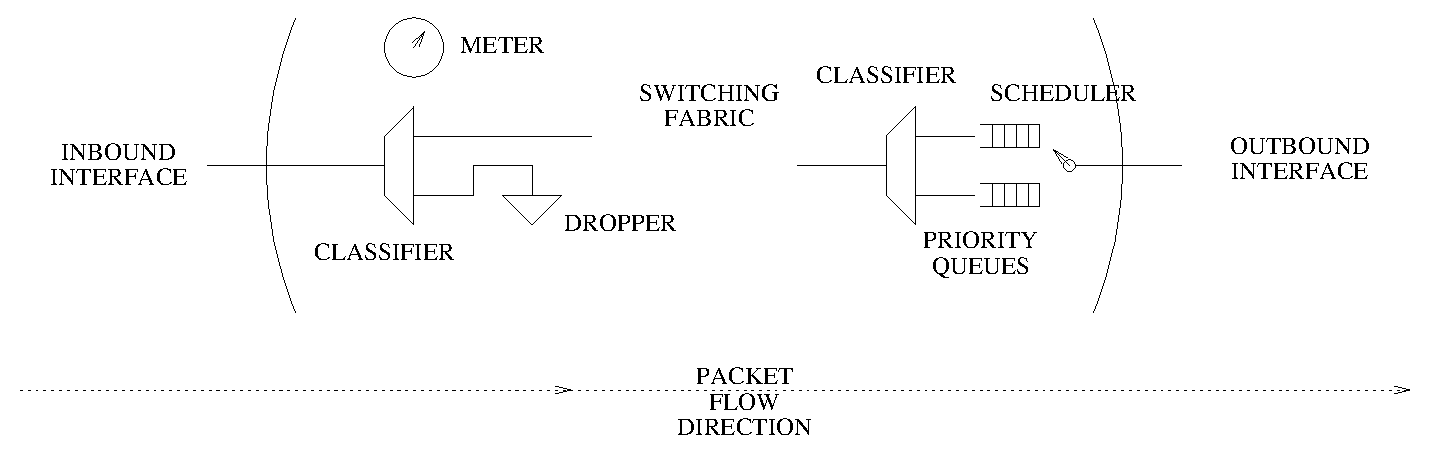
\includegraphics[width=\linewidth]{figures/qos_chain.eps}
\caption{QoS tools chain of the inbound and outbound interface of a router.}
\label{fig:qos-chain}
\end{figure}

\subsection{Classifiers}

To apply QoS, it is required to discriminate among different classes of traffic.
Therefore, the first step in any QoS tool chain is always classification.
This classification is performed by a tool that we call classifier.

These are some of the classification criteria that can be applied by a classifier:
\begin{itemize}
\item Incoming interface: Packets can be classified using the interface (either physical or virtual) that they are coming from.
As an example, we can have all the IP phones in our network in the same VLAN, and then classify the packets of this VLAN as expedited forwarding (EF).

\item Metering: We can take a classifying decision based on traffic volume.
This is typically done with token buckets (e.g. RFC 2698 \cite{rfc2698}).
Traffic conforming to a token bucket of a given rate and burst size receives a different classification than non-conforming traffic.
It is also possible to classify the traffic in three different colors (green/yellow/red) according to the CIR/PIR criteria.

\item QoS fields: We have mentioned that IP, Ethernet and MPLS packets all have a field for QoS.
The bits (the marks) in these fields can be used for classification purposes.

\item Other headers: The other headers of the packets can also be used for classification purposes.
For example, if we have a server devoted to VoIP services, we can prioritize all the packets destined to (or originated from) that server.

\item Deep packet inspection: This involves opening the packet and looking into its contents to take a decision.
It can be useful to detect signatures of virus, and identify higher layers protocols.
In the field of QoS, it is used for example to classify P2P traffic (bittorrent, kazaa).

DPI is also used for security, surveillance, espionage and censorship purposes.

\item Stateful inspection (SI): In stateful inspection we use not only information in the packet, but also information of previous packets.
As an example, it can be used to identify encrypted P2P traffic by identifying patterns such as communications with many other devices taking both the role of client and server.
\end{itemize}

DPI and SI are computationally expensive.
It would be desired to perform them only once, rather than repeating the effort in every router.
The problem is that all the classification effort is lost after the packet leaves the router, unless the QoS headers are explicitly changed.
In the next subsection we introduce the marker, which is the tool that changes QoS markings.

\subsection{Markers}

Classifying can be computationally expensive.
Additionally, some classifications can be done only at the entry point of the network.
As an example, imagine a classification based on a metering tool for the traffic of a given client.
It is feasible to use the metering tool and the classifier in the interface that the client uses to connect to the network.
However, after that traffic has been aggregated with traffic of other customers, it might not be possible isolate it with the purpose of metering.
In core routers with the larger line-speeds, only very simple (hardware based) classifications are possible.

For all these reasons, it is necessary that the routers can pass some information to each other regarding classification.
The tool for this is the marker, that changes the bits of the QoS headers of the packets.

\subsubsection{Where to classify and mark?}

Classification is done in the entry point of the network, which is also called the trust boundary.
If a network wants to identify P2P traffic to throttle it down, it will do it at the edge routers, which are the first routers that have the opportunity to inspect the packets.
Then, the QoS field of the packet headers will be marked so that other routers of the network don't have to repeat the expensive classification process.
The classification done by the other routers will be straightforward as all they have to do is to check the QoS field.

The volumes of traffic in edge routers are smaller than in core routers.
Edge routers have the necessary time to classify and mark the packets.
Edge routers also can easily differentiate traffic of different customers for metering purposes.

This initial marking may also be accompanied by policing.
A common example is to classify the traffic coming from a customer into three colors in the edge router.
Green packets are the ones conforming the CIR.
Yellow packets are the ones conforming the PIR.
And Red packets are the ones exceeding the PIR.

Red packets will be dropped (policed).
Yellow packets will be marked for drop precedence.
And green packets will be forwarded unmarked.
In case of congestion, yellow packet will also be dropped.

If the yellow packet that has been marked for drop precedence continues its trip towards its destination, it may be the victim of active queue management (AQM) tools at some later point.

\subsection{Policers}

Policers combine a meter and a dropper.
The meter is a classifier that has been explained before, and the dropper simply drops packets.
Policers play a role in enforcing CIR/PIR agreements and also in guaranteeing bounded delay for packets traversing the network, and a fair bandwidth distribution.

If an SLA defines a PIR and the customer sends traffic exceeding the PIR, the ISP will police the exceeding traffic.
A reasonable customer might police the traffic himself, to select which are the less important packets and avoid that the ISP drops packets.
Another alternative is that the customers shapes its traffic.
We will cover shapers in a later subsection.

Policers can also be used before queues.
By controlling the input rate and the size of a queue (or a set of queues) it is possible to provide delay and bandwidth guarantees to each queue.

As an example, if a queue for VoIP packets is serviced at a rate of 100 Mbps and the input is policed at a rate or 1 Mbps, with a bucket size of 100 Kbits, the  delay is bounded to $\frac{10^5 bits}{10^8 bps} = 10^{-3}s$.
Note that the delay guarantee is derived from the bucket size and not from the rate.

The rate limit is important when the voice queue is prioritized over other queues.
If the priority queue is not policed, it can starve other queues in case of misbehaviour.

Note that policers introduce packet drop but don't introduce delay.
There is a token bucket that stores tokens, but not packets.
The next subsection introduces traffic shapers that can prevent packet loss at the expense of delay.

\subsection{Shapers}

We have seen that policers drop traffic that does not conform to a given traffic profile.
An alternative of dropping is buffering.
When a shaper receives a packet and there is not enough tokens in the bucket to serve it, it will store it in a queue.
As soon as there are enough token in the bucket to serve the first packet of the queue, the shaper will allow the first packet of the queue and decrement the number of tokens in the bucket accordingly.

As the buffer size is finite, it is possible that the buffer fills up and the shaper loses packets.

Shapers are normally not appropriate for VoIP, as they introduce delay.
However they can be used to set the pace of TCP flows effectively and for this reason it is said that they are TCP friendly.

By holding packets in the buffer, the shaper increases the RTT delay.
The result is that the TCP rate is slowed down.
In the event that the buffer fills and a packet is lost, TCP halves its transmitting rate.
However, as the buffer is full, the shaper keeps transmitting at a full rate for some time and gives time to TCP to build up the congestion window and increase the transmitting rate again.

An alternative implementation of the shaper is to use a leaky bucket instead of a token bucket.
The leaky bucket simply stores packets and ``leaks'' them at a given rate.
Therefore, the leaky bucket does not allow any kind of traffic burstiness.

\subsection{Queues, droppers and schedulers}

This is a critical component of QoS.
Packets are stored in one or more FIFO queues and there is a scheduler that ``serves'' the queues by taking the first packet of a queue.
Another element of the system is the dropper, that drops packets.

There are several alternatives for the implementation of the scheduler and the dropper and we will discuss them in the next chapter.

We want to mention here that the queues do not usually contain the packets as it is much more effective to store pointers to the packets.

\subsection{The TX-ring and the interleaver}
The last element of the tools in router, just before the transmission line, is the transmission ring (TX-ring).
The normal configuration is having a queue system and the scheduler taking packets from the queues and placing them in the TX-Ring.
Differently from the queues, the TX-ring does not contain a pointer to the packet.
It contains the actual packets, ready to be transmitted.
The goal of the Tx-ring is to feed the transmission line, to make sure that it is continuously transmitting if there are packets to be serviced.
The Tx-ring is normally dimensioned in such a way that there is at least the packet that is currently under transmission and one additional packet that will follow.

The TX-ring is completely FIFO and there is no possibility to apply prioritization over the packets when they reach it.
This is not a problem in high-speed transmission lines, when transmitting a packet takes less than a millisecond.
However, in low-speed lines, the packets stored in the TX-ring can substantially delay a high priority packet.

Consider the following example.
A router transmits two kinds of traffic: VoIP and backup data.
VoIP are short (100 bytes, 800 bits) and have strict priority over backup packets, which are long (1500 bytes, 12,000 bits).
At a given point of time, the VoIP queue is empty and therefore the scheduler serves packets of the low priority queue.
The low priority queue may have a large number of packets (let's say 10) but the scheduler makes sure that there are not more than two packet in the Tx-ring.
We have a situation in which we have two long packets in the Tx-ring and a VoIP packet arrives to the high priority queue.
The VoIP packet has priority and therefore it will be the first one to be served by the scheduler.
Still, it will have to wait for the two long packets in the Tx-ring which have already been served by the scheduler.

Transmitting two 12,000 bits packets over a 1Mbps line takes around 24 ms, which is a substantial delay for VoIP packet.
To prevent this problem, an interleaver can be used in low speed link.
The idea is that long packets are divided in smaller ``chunks''.
Then, the scheduler serves chunks of a packet, instead of the whole packet.
This approach reduces the delay and jitter for high priority traffic.

\chapter{Scheduling}

Scheduling is a key tool in QoS and it is complex enough to deserve its own chapter\footnote{A word of warning is needed. In different books, articles and information sources, different names are used for the same scheduling techniques. To add to the confusion, a same technique name has different meanings when looking at different sources.}.
A scheduler serves two or more queues and has to take decissions about which queue has to be served first.
The combination of queues and scheduler can change the order of the packets.
For this reason it is important that all packets of a same flow are mapped to the same queue, to prevent packet re-ordering.

\section{Strict Priority Queues}

Prioritizing is a core idea in QoS.
Imagine that a big packet belonging to backup tool such as Dropbox arrives to a router.
Right after that, a second packet arrives to the same roter.
Imagine that this second packet is a small VoIP packet.

The VoIP packet is in a hurry, because it must make it to the decoder before the playout time.
For this reason, the combination of queues and scheduler will allow the VoIP packet to advance the backup packet and be transmitted in the first place.

In the simplest case we have only two queues: the high priority queue and low priority queue.
A classifier maps each of the packets to one of the queues.
The scheduler will serve the high priority queue whenever there is a packet in that queue.
Only when the high priory queue is empty, the scheduler will serve the low priority queue.

Note that this concept can be easily generalized to the case in which there are more than two queues.
The principle is that a queue will be served only when all the higher priority queues are empty.

\subsection{Preemptive strict priority}
In preemptive strict priority, if a high priority packet arrives while a low priority packet is being served, the service of the low priority queue is interrupted and the high priority packet is served immediately.
Theoretically, the service of the low priority packet is resumed when the high priority queue becomes empty.

This approach is very beneficial for high priority packets as they are never disturbed by low priority packets.
The only problem with this approach is that, in practice, it is not trivial to stop a transmission of a packet and later resume it.

\subsection{Non-preemptive strict priority}
In non-preemptive strict priority, if a high priority packet arrives while a low priority packet is being served, the transmission is not interrupted.
The high priority packet will wait for the transmission of the low priority packet to finish and then it will be transmitted.

This is the approach that is used in practice in high speed transmission lines.
The problem with this solution is that, in a slow transmission line, a high priority packet might need to wait for a long time if it arrives while a long low priority packet starts being serviced.

\subsection{Fragmenting and interleaving}
An intermediate solution between the two mentioned before is fragmenting each packets in chunks and serving one chunk at a time. 
Using this technique we can emulate a behaviour similar to preemptive strict priority.
As it has been explained in the previous chapter, fragmenting and interleaving are used in low speed lines.

\subsection{Starvation and policing}
The problem of strict priority queueing is that the high priority queue can easily eat up all the bandwidth.
If there are always packets in the high priority queue, the other queues will never be serviced.
This might be an undesirable situation.

In the following we will review other queueing strategies that avoid this problem.
Nevertheless, priority queueing is still used for real-time traffic such as VoIP, as it minimizes the delay for high priority traffic.
The solution to prevent starvation, is two police the high priority queue.

The high priority traffic is policed before entering the queue to a fraction of the total bandwidth available in the interface (e.g., 10\% or 30\%).
By doing so, the other queues are safe from starvation.
Even if a virus, a worm, or a misconfigured generates a low of high priority traffic, it will not kill the network.

\section{Round Robin Scheduling and Weighted Round Robin}

One of the most direct ways of sharing the available bandwidth among different queues is to serve one packet of each queue at a time in order.
As an example, if there are three queues, a round robin (RR) scheduler will serve Q1, Q2 and Q3.
And then again Q1.

If one of the queues is empty, it is simply skipped.
This property is called the work-conserving property, and guarantees the full utilization of the link while there are packets waiting.

If we want to prioritize Q1 over Q2 and Q3 and Q2 over Q3, we can configure the scheduler to serve the queues in this order: Q1, Q2, Q1, Q3, Q1, Q2.
And then repeat the same schedule again.
Note that with this particular schedule, Q1 is served thrice in each round, Q2 is served twice and Q3 is served once.
This particular approach in which different queues have different weights is called Weighted Round Robin (WRR)

Round robin is flexible and precise when it comes to adjust the number of packets transmitted by each queue.
The actual bandwidth allocated to each queue depends on the schedule, but also on the length of the packets.

Recovering our example of three queues, if the packets in Q3 are 12000 bits long and the packets of Q1 are 200 bits long, Q3 will receive twice as much bandwidth as Q1.
If we want to allocate a fraction of the available bandwidth to each of the queues and we don't know the length of the packets in advance, it will be impossible to use WRR.

\section{General Processor Sharing}

General Processor Sharing is an idealized sharing approach that assumes a fluid model.
It assumes that the scheduler can serve an infinitesimal amount from each of the queues.
It is easy to imagine with the example of liquid reservoirs instead of queues, and pipes draining liquid from each of the reservoirs.
One pipe may be draining one liter per hour and the other two liter per hours.
Still, at any given point of time, both reservoirs are drained simultaneously, even though one is served twice as fast as the other.

In the practice of packet networks, it is not possible to implement this idealized model.
An approximative implementation is used and we explain it in the next section.

\section{Deficit Weighted Round Robin}

In deficit Weighted Round Robin (DWRR) each queue has an associated ``token bucket''.
It is called the ``deficit counter'', and it is measured in bytes.
The scheduler visits all the queues, one by one.
In every visit, the scheduler increases the deficit counter by a value which is called ``quantum''.
If the value of the deficit counter after being increased is larger than the size of the first packet in the queue, the packet is served.
The deficit counter is decreased by a value equal to the size of the packet that has been served.
If, after being decremented, the deficit counter is larger than the size of the following packet, another packet is served and the deficit counter is decremented accordingly.
This process is repeated until the deficit counter is smaller than the first packet of the queue or the queue is empty.
In the former case, the value of the deficit counter is saved for the next round.
In the latter case, the value of the deficit counter is reset.
At this point, the scheduler moves on to serve the next queue.

By adjusting the quantum of each queue, we can set the weight (in terms of bandwidth) of each of the queues.
As an example, if we set a quantum of 400 bytes for the high priority queue and a quantum of 200 bytes for the low priority queue, the high priority queue will receive twice as much bandwidth.

Let's look at an example.
The high priority queue contains a 500 bytes packet, and the low priority queue a 400 bytes packet.
Both deficit counters are zero.
In the first round, the deficit counters are incremented to 400 and 200, and no packet is served as the values of the counters are lower than the size of the packets.
In the second round, the counter of the high priority queue is incremented to 800.
The first packet is serviced and de counter is decremented to 300.
While the first packet is being serviced, a 100 bytes packet and a 500 bytes packet arrive to the high priority queue.
When the service of the first packet finishes, the deficit counter of the first queue (300 bytes) is larger than the size of the head-of-queue packet (100 bytes).
Consequently, the head-of-queue packet is served and the deficit counter is decremented to 200.
At this point, the counter is smaller than the size of the head-of-queue packet and therefore the scheduler jumps to the next queue.

It increases the counter of the second queue by 200, and the resultant value (400) is equal to the size of the head-of-queue packet of the second queue.
This packet is being served and the counter decremented.

The scheduler moves to the first queue again, it increases the counter by the quantum (400) to 600.
Then it serves the head-of-queue packet, which has 500 bytes, and decrements the deficit counter by 500.


\chapter{Active Queue Management}

In Chapter \ref{cha:quality_metrics} we mentioned that some of the Internet applications are elastic in the sense that they make use of all the available bandwidth.
The interesting part is that these application don't know in advance how much bandwidht is available, which means that they have to find it out somehow.
In this chapter we describe how TCP congestion control and Active Queue Management (AQM) work together to throttle bandwidth hungry applications.

The interplay between TCP and AQM is critical to deliver satisfactory performance.
In 2009, mainstream media\footnote{E.g. www.nytimes.com/2009/09/03/technology/companies/03att.html} reported performance problems in AT\&T's wireless data network.
The alleged cause was the increase of data usage due to the popularity of IPhones.
The underlying reason seamed to be a poor buffer dimensioning\footnote{http://blogs.broughturner.com/2009/10/is-att-wireless-data-congestion-selfinflicted.html}.

\section{TCP congestion control}
We will introduce the working principles of TCP.
This is not meant to be an accurate description of TCP, just an overview of the concepts used for congestion control.
TCP is indeed very complex, heterogeneous (different in different OS) and continuously evolving.
An accurate description of TCP is beyond the scope of this course.

TCP is a flow-oriented transport (layer 4) protocol that is used by the elastic applications in Internet.
This includes most of the applications, such as web browsing, email and file transfer.
Take the example of a large file transfer using FTP, which involves the transmission of a large amount of data.
TCP doesn't know how much bandwidth is available, so it will start transmitting one packet.
If this packet is successful, it will transmit two packets.
These two packets represent, the amount of unacknowledged data on-the-fly and this limit is called the congestion window.
And if these to packets are positively acknowledged, TCP will duplicate its congestion window one more time and send four packets.
This process is called the slow start phase of TCP.
Even though it starts slow, the true is that it is growing exponentially and, at some point, the transmitting rate will exceed the available capacity and a packet will be dropped.

When TCP detects that a single packet has been dropped (signaled by a duplicate ack), it halves its congestion window and starts increasing it linearly at a rate of one MTU for RTT.
This phase is called congestion avoidance, as TCP slowly grows its congestion window trying to find the limits of the available capacity.
If another packet loss occurs which results in another duplicate ack, the congestion window is halved again.
The result is that the sending rate of TCP approaches the available capacity.

If the loss of a packet is detected due to a timer timeout, TCP assumes that something is very wrong with the network and moves back to the initial slow start behaviour.

In summary, TCP will always try to increase its sending rate.
Only when a packet is lost, TCP will reduce its sending rate as the packet loss is interpreted as a sign of congestion.
Therefore, in principle, it is necessary to drop packets to signal TCP to lower its sending rate.

\section{Long Fat Networks}

As the bandwidth of the Internet lines increase, TCP needs to keep up with this progress and be able to fill this pipes.
If you have a high-speed connection (say 1 Gps) and a long end-to-end delay (100ms), you need a lot of data to fill it.
In this particular example, 100 Mbits of data are needed to fill the pipe.

If TCP does not fill the pipe, and pushes only 1 Mbit of data in it, then it is wasting 99\% of the available bandwidth.
For this reason, modern operative systems use techniques (basically, window scaling) that make it possible to push much more data into the pipe than the original TCP, which allowed only for 64 Kbytes.


\section{Bufferbloat}

It can be tempting to dimension a buffer so that there is no packet loss.
However, increasing the buffer size can increase the delay to unacceptable limits.
This problem seems to be prevalent in today's Interned, and has been termed ``bufferbloat''.

\subsection{Good Queues and Bad Queues}
Queues play a critical role in data packet networks.
They absorb a temporal burst and smooth it out for transmission over a line.
The burst can be caused by bursty sources and also by statistical multiplexing.
A good queue absorbs the burst, fills it up, and then empties completely.

But there are also bad queues.
Bad queues are full for a long time.
Note that a queue that is full for a long time is not useful for absorbing bursts (as it is full and cannot absorb anything) and it has the negative effect of increasing delay.
Bad queues appear frequently when there is a high-speed to low-speed transition.

A good example is a 1 Gbps home network that connects to an ADSL which can upload 2Mbps.
If you start to upload a large file to the Internet, TCP will do its best in ``filling the pipe'', and the effect of that action would be to fill the buffer of the ADSL router.
If that router has a large buffer, it will introduce a lot of delay.
TCP will believe that it is dealing with a ``long pipe'', as the delay is long, and will persist in the efforts of filling it.

The result is an artificially bloated delay, which not originated by the long distance, but by the large full buffers.
A large full buffer does not provide any benefit to the network, other than unnecessarily increasing the delay.
Delays of several seconds have been reported due to bufferbloat.

It is important to realize that large buffers may have the effect of penalizing the network performance.

\section{Taildrop and Weighted Taildrop}

In the good old times, high speed memory was expensive and therefore the amount of it in routers and other switching devices was limited.
Consequently, the queues were not very large because there was no room to store a lot of data in the router.
As memory got cheaper, manufacturers beefed up their devices with more memory.
This turned out not to be an improvement on the network performance, as larger buffers resulted in ``bufferbloat''.

It is obvious that it is good to keep queues to a limited size, e.g., to avoid infinite queues.
A first possibility, is to have a queue size and drop packets that arrive when the queue is full.
This approach is called taildrop, as packets are dropped from the tail of the queue.

The size of the queue can be measured in packets, in bytes or in milliseconds.
To make the measure in time, we need to take into account the speed of the interface.
This is normally a good idea, as the amount of data that needs to be buffered is closely related to the speed  of the line.
Expressing the queue length in time also gives a direct idea of the delay that can introduce de queue.

As an example, a 10 ms queue size seems to be a fair size for many applications.
A 10 seconds queue is probably excessive for many applications, such as web browsing.

In the simplest approach, all the packets arriving to a taildrop queue are subject to the same restrictions.
If the queue is full, the packet is discarded.
Otherwise, it is accepted.

It is possible to refine this approach taking into consideration QoS differentiation.
Imagine that in a previous stage we have marked packets as being either in-contract or out-of-contract.
Then we can set two different queue sizes for different packets.
We can accept in-contract packets if the queue size is below 10 ms and out-of-contract packets if the queue size is below 5 ms.
In this case, out-of-contact traffic has a higher dropping precedence that in-contract traffic, and we lessen the extent to which in-contract traffic can be delayed (or even dropped) due to out-of-contract traffic.

The technique that uses different queue sizes for different packets is called weighted tail drop.

\section{TCP global synchronization}

Another event that penalizes network performance is TCP global synchronization.
It occurs when a tail-drop queue accommodates packets of several TCP sessions.
The TCP sessions keep increasing their congestion windows and transmission speed until the queue fills up.
At this point, the tail-drop queue drops all the arriving packets.

All the TCP sessions detect packet loss and halve their sending rate simultaneously.
As a result, the queue empties and then the link remains unused for some time.
Then the TCP sessions starts growing again, and the story repeats one more time.

Observe that bufferbloat and TCP global synchronization are complementary problems.
In the former, the queues are empty.
In the latter, the queue is empty for a substantial fraction of time.
Ideally we would like that there was always a packet ready to be transmitted, to take full advantage of the link capacity.
Simultaneously, we would like that there was only a single packet, as the presence of many packet introduces unnecessary delay.

Active queue management (AQM) addresses tries to address these problems.

\section{Random Early Detection}

A first approach to prevent that queues fill up and the bufferbloat and TCP global synchronization problems appear, is to start discarding packets before the queue is full.
The general idea is to accept all packets when the queue is empty (or almost empty), some packets as the queue starts to fill up, and all packets when the queue is full (which should not happen).
Packet loss is induced deliberately before the queue is full to signal the involved TCP flows that they should reduce the sending rate.
The big difference is that not all the flows receive this signal simultaneously.
With RED, the packet drop is distributed evenly in time, so that the TCP halve their transmission rates at different instants and therefore the aggregated sending rate evolves smoothly in time.

By avoiding the sharp drop of the aggregated sending rate in TCP global synchronization, it is possible to achieve a better utilization of the available bandwidth\footnote{Cisco provides a figure supporting this statement in http://www.cisco.com/image/gif/paws/10582/60c.gif}.


The first step to implement RED in a router is to compute the average delay\footnote{Note that recent papers point out that average queue delay is not a relevant metric to differentiate between good queues and bad queues \cite{nichols2012cqd}.}.
This is computed using an exponential weighted moving average with parameter $w$.
The current average $q_{avg}$ is computed using the previous average value $q_{prvavg}$, the last measured value $q_{measured}$ and the parameter $w$ as follows.
\begin{equation}
q_{avg} = \frac{2^w-1}{2^w}q_{prvavg} + \frac{1}{2^w}q_{measured}
\end{equation}

If $q_{avg}$ is below a minimum threshold ($q_{min}$) the packet is always accepted.
If $q_{avg}$ is larger than the maximum queue length $q_{max}$, the packet is rejected.
In the case that $q_{min} \leq q_{avg} \leq q_{max}$, the packet is accepted with probability
\begin{equation}
P[packet accepted] = \frac{q_{avg}-q_{min}}{q_{max}-q_{min}}P_{max},
\end{equation}

where $P_max$ is yet another configuration parameter that determines the dropping probability when $q_{avg}$ approaches $q_{max}$ from the left.

It is straightforward to generalize RED to weighted RED in which different packets use different profiles (different configuration parameters) in order to prioritize some packets over the others.
Typically, packets with higher dropping precedence are exposed to more aggressive RED profiles.

\section{Explicit Congestion Notification}

It is sad to drop packets when they are half-way towards their destination, but in principle it is the only mechanism to signal TCP that it has to reduce its sending rate.
There is an alternative, introduced in  RFC 3168 \cite{rfc3168} which allows notifying TCP without dropping packets.

First it is necessary that both communication endpoints can support ECN and agree to use it.
If they do, they will the least two significant bits of the DiffServ field to indicate it.
These bits will be set to either 10 or 01 if ECN is being used, and 00 otherwise.

If a that supports ECN decides to drop a packet, it will first check whether the packet belongs to a flow that supports ECN.
If it does, it will set the ECN bits of the packet to 11 and will not drop the packet.
The receiving host will use some flags on the TCP headers to signal the originating host that the network is congested.

Upon reception of this signal, the originating host will reduce its congestion window (and thus its transmitting rate) just as if a packet dropped has occurred.
The advantage is that there is no need for packet re-transmission.
This way, it is possible to achieve congestion control without packet dropping.

\section{CoDel}
The latest trend in AQM is Controlled Delay (or CoDel) \cite{nichols2012cqd}, which discards packets when the minimum queue occupation exceeds a threshold (in time).
This technique seem to be easier to configure and provide better link utilization while preventing bufferbloat.

\chapter{Differentiated Services}

The IETF has proposed two main solutions for the Internet QoS architecture: Integrated Services and Differentiated Services \cite{rfc2475}.
The first one implies per flow signaling and reservation, and therefore it does not scale well in large network.
The focus of this chapter is on the second alternative.
In differentiated services, traffic is classified in a reduced number of classes, typically less than eight.
The routers implement different PHB for the different classes, which provides the desired QoS.

Note that since in Diffserv there is not a per flow signal and admission control, in principle it does not guarantee that the QoS requirements are actually satisfied.
In reality, this is achieved with a combination of traffic conditioning at the edge of the network and capacity planning.
This is not an exact science, but we'll cover the basics through examples and typical configurations.

\section{Key aspects of DiffServ}
DiffServ is an scalable solution for QoS provisioning in IP networks.
DiffServ offers the tools for network administrators to implement QoS in an IP domain.
This can be used to offer VPNs that satisfy SLAs and to support services with tight QoS requirements such as VoIP.

The interconnection of different DiffServ domains is somewhat more complicated, as needs the collaboration of the different organizations that manage the different networks.
DiffServ is not commonly used for generic Internet access, as the Internet involves a humongous collection of networks which makes the provision of QoS guarantees an enormous challenge.

Three key aspects of DiffServ are border traffic conditioning, DiffServ markings, and PHBs.

\subsection{Traffic Conditioning}

Together with the SLA, a traffic conditioning agreement (TCA) is also established.
The TCA is often defined as a packet marking combined with token bucket bucket, of a given rate and depth.
For example, it may specify that packets with VoIP traffic will conform to a token bucket of rate 1Mbps and depth 1Kbps.

At the edge of the network, the routers will perform classifying, metering and policing to ensure that the offered load complies with the specified TCA.
The traffic exceeding the TCA may be either dropped or marked as non-conformant.

As the tasks of classifying, metering and policing require computational resources, they are done only at the edge.
At the edge of the network line speeds are lower than in the core of the network, and therefore it is possible for the router to process all the packets.
In the core of the network, the switching speeds are much higher and the time required to process each packet should be minimized, and therefore there is no time for classification, metering and policing.
As the edge of the network grows when the network grows, this solution is scalable and therefore appropriate for large networks with large volume of traffic.

According to the initial classification, the edge router will mark the packets using a field in the IP header which is the DiffServ Code Point (DSCP).

\subsection{DiffServ Code Point}

The DiffServ is a 6 bits field in the IP header that is assigned to each packet in the edge of the network.
The DSCP assigns a packet to one of the possible traffic classes supported by the network.
There are some standardized values for this field, such as Expedited Forwarding (EF), that we will review later.
But its value is of significance within the DiffServ domain and therefore the network administrator have the decision of which DSCP values are used and what is the meaning of each of them.
This marking can be used later by the other routers of the network to quickly classify the packet, and treat the packet in accordance of the traffic class to which it belongs.
This treatment is the per-hop-behaviour (PHB).

\subsection{Per Hop Behaviour}

For each of the traffic classes (DSCP values) supported by the network there has to be an associated PHB.
This can be a many-to-one mapping, as different DSCP values can be offered the same PHB.
The PHB is a high level description of the service that a packet will receive when it arrives to a router.
It does not detail the QoS tools that will be used to implement that behaviour.

\section{IETF defined per-hop-behaviour}
The IETF has provided recommendations for four PHB.
A recommendation combines a description of the PHB with a suggested DSCP.

\subsection{Default PHB}

It is a required behaviour and it is assigned the DSCP 000000BIN.
RFC 4594 \cite{rfc4594} specify that there is typically some bandwidth guarantee for this kind of traffic, but the packets can be lost, reordered, duplicated or delayed at random.

\subsection{Expedited Forwarding (EF)}
Expedited Forwarding (EF) is defined in \cite{rfc3246} and uses the code point 101110BIN (46DEC).
The purpose of this PHB is to serve real-time traffic such as VoIP or videoconferencing.
It should provide guaranteed bandwidth with low delay, jitter, and packet loss.

This can be attained by using strict priority queueing in combination with a buffer that is large enough to accommodate the traffic bursts.
The traffic is policed to control its rate and burstiness.
The rate needs to be controlled to ensure that this priority traffic does not starve other classes of traffic.
The bucket depth needs to be smaller than the allocated queue space, to guarantee that no packet loss will occur due to full queues.
The depth is also important as it determines the maximum delay that a packet may suffer, which is the token depth divided by the transmission rate.
The maximum delay obviously also influences the maximum jitter that the packets will suffer.

\subsection{Voice Admit (VA)}

Similar to EF, with the difference that Voice Admit (VA, \cite{rfc5865}) is subject to a call admission control procedure.

\subsection{Assured Forwarding (AF)}

Assured Forwarding is actually a group defined in \cite{rfc3260} that comprises 12 DSCPs.
The packets belonging to this group will be forwarded is the offered rate is kept below the committed rate.
It differentiates four different classes: AF1x, AF2x, AF3x and AF4x.
AF1x is the lowest priority and AF4x is the higher priority.
A typical implementation is to assign each of the classes to a queue and use DRR to distribute the bandwidth among the classes.

Within each of the classes, there are three possible drop precedences.
As an example, we have AF11, AF12 and AF13.
This means that, if congestion occurs, AF12 packets will be dropped with higher probability than AF11 packets.
And AF13 packet will be dropped with higher probability than AF11 and AF12 packets.

A typical scenario is to use a two-rate meter within a class.
If we take AF1x as an example, in-contract traffic is assigned to AF11, out-of-contract traffic is assigned to AF12, and traffic exceeding the PIR is simply dropped.

AF11 and AF12 will be mapped to the same queue.
This is an important aspect as otherwise packet re-ordering may occur.
Then, different RED profiles will be applied to AF11 and AF12.
AF12 will suffer a more aggressive RED profile to ensure that out-of-contract packets are the first to be dropped.

\subsection{Class Selector (CS)}
This was included to provide some kind of backward compatibility with pre-DiffServ approaches.
The first three bits (0-2) to indicate precedence: higher value means higher precedence.
A practical use is to ease mapping from IP QoS markings to EXP QoS markings.


\subsection{Differentiated Services in MPLS}
In MPLS there are only three EXP bits for QoS markings.
If the ``class selector'' PHB are used, which use only the first three bits of the six available in DSCP, it is very easy to map from DSCP to EXP and the other way around.
All is needed is to copy those three bits when an IP packet enters the MPLS domain.

If ``class selector'' is not used, but there are less than eight different classes, it is still possible to map from DSCP to EXP.
This would be the case if AF11, AF12, AF21, AF22, AF31, AF32, AF41 and AF42 are used.
The approach in which the information about the traffic class is contained in EXP bits is called EXP inferred PHB selection (E-LSP, where LSP stands for label switched path).

If the classification used has more than eight different DSCP values, a first option is to opt for a many-to-one mapping.
As an example if the eight classes mentioned above are used and in addition also EF is necessary, a possible option would be to treat AF1x packets just as AF2x packets.

An alternative to the many-to-one mapping is to use the label for QoS.
In our example, we could use five different labels.
One for each of the AF1x groups and the fifth one for EF.
When the LSP identifier carries QoS information it is called label inferred LSP (L-LSP).


\begin{appendices}
\appendixpage
\noappendicestocpagenum
\addappheadtotoc

\chapter{Lab Assignments}

In these labs you can use any programming language that you want. 
In each assignment you must deliver the source code and a brief explanatory pdf document explaining how you solved the assignment.
It should also include some examples, including the commands that you used to test it and the results.
Some assignments may ask for additional information, such as plots.

Pack all the files in a zip file (not rar) and submit it using moodle.
Remember to include the names and NIA in all the source files and in the document.

Prepare the assignment in advance, so that you can complete it during the class.
The submission deadline will be one week after the class.

\section{Traffic Generator and Sink}

In this lab assignment you will program a Poisson traffic generator and a traffic sink.
The Poisson traffic generator takes the following parameters:
destination host, destination port, packet rate and traffic class.

It generates UDP packets with a string that contains three integer values separated by a blank space. The integers represents a packet id (starting with 0), time stamp in milliseconds (local significance only) and traffic class.

The traffic sink takes a port number as a parameter and computes packet delay and packet loss for each packet class (computation of jitter is optional).

Test it with a traffic generation rate of 10 packets per second.

Note that since the generator and the sink are directly connected, the delay, the jitter and the packet loss will will be zero.

In the next assignment we will place a queue in between.
Then these values will no longer be zero.

\begin{figure}[!h]
\centering
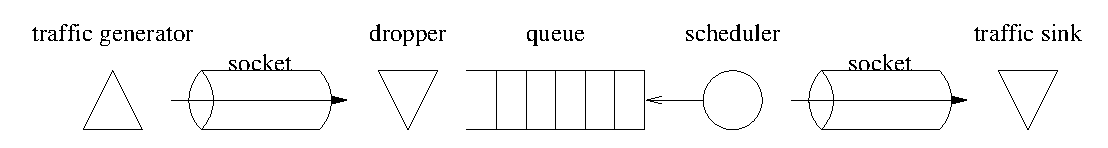
\includegraphics[width=\linewidth]{figures/scenario.eps}
\caption{Scenario to test in lab assignment.}
\label{fig:scenario}
\end{figure}

\section{A queue}

The second module that you have to construct in this course contains a queue (that includes a dropper a buffer) and a scheduler.

Note that each module has to be a separate program. The different modules communicate (send packets to each other) using sockets.

This program listens at an udp port and transmits the packets to a given udp port and address. Consequently, it has to be simultaneously an UDP server and an UDP client. You may consider the possibility of using different threads for the dropper and the scheduler.

All port numbers and the destination should be configurable as parameters. An additional parameter will configure the queue size (number of packets). If the queue size is set to zero, it means infinite queue length. If a finite queue is used, a taildrop policy will be applied.

The scheduler should be configurable to be able to choose an exponentially distributed service time or a deterministic service time. In either case, the service rate should be taken as an input parameter.

Combine the Buffer with the traffic generator and traffic sink modules to make measures of packet loss and delay.

\begin{figure}[!h]
\centering
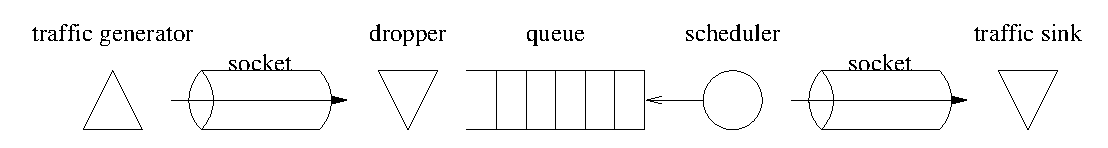
\includegraphics[width=\linewidth]{figures/scenario2.eps}
\caption{Scenario to test in lab assignment 2.}
\label{fig:scenario2}
\end{figure}

\section{Priority Queues}
The third module that you have to construct in this course contains two priority queues (that include a dropper a buffer) and a scheduler.
We will name $H$ the high priority queue and $L$ the low priority queue.

Each module has to be a separate program. The different modules communicate (send packets to each other) using sockets.

This program listens to two udp ports and transmits the packets to a given udp port and address. Consequently, it has to be simultaneously an UDP server and an UDP client. You may consider the possibility of using different threads for the droppers and the scheduler.

The scheduler strictly prioritizes queue $H$.
That is, it starts to serve queue $L$ only if there are no packets at queue $H$.
Nevertheless, this is non-preemptive priority, which means that the server will not interrupt a service to queue $L$ when a packet arrives to queue $H$.
The server will complete the service to the packet of queue $L$ and only then it will serve the packet that has arrived to queue $H$.

All port numbers and the destination should be configurable as parameters. An additional parameter will configure the queue size (number of packets). If the queue size is set to zero, it means infinite queue length. If a finite queue is used, a taildrop policy will be applied.

The scheduler will draw service times from an exponential distribution.

Combine the priority queues with two traffic sources that generate different classes of traffic and obtain statistics of the delay for each of the traffic classes.

\begin{figure}[!h]
\centering
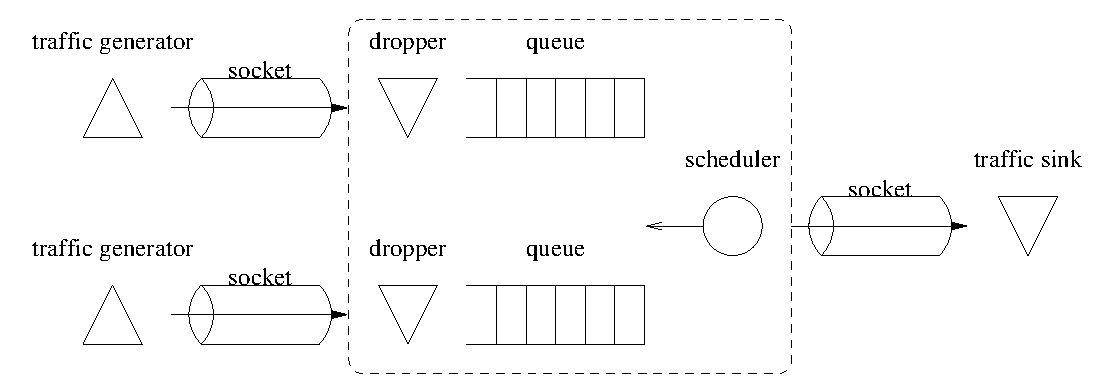
\includegraphics[width=\linewidth]{figures/scenario3.eps}
\caption{Scenario to test in lab assignment 3.}
\label{fig:scenario3}
\end{figure}

\section{Optional QoS Tool}

In this lab assignment you will implement one ore more QoS tools of your choice.
You can choose any of the following tools that we have seen in class: classifier, metering, token-bucket policer, leaky bucket shaper with RED, re-write.

A brief description of each of the tools follows:
\begin{itemize}
  \item{classifier:}
  It has an input socket and several output sockets (one for each possible class of service).
  The classifier checks the class of server marking of the packet and redirects the packet accordingly.
  \item{metering:}
  It has an input socket and three output sockets.
  It uses two token buckets (as described in rfc2698) and it takes as an input four parameters: CIR (packets per second), PIR (packets per second), CIR burst (packets) and PIR burst (packets).
  The green, yellow and red packets are sent to each of the three different output sockets.
  \item{token-bucket policer:}
  It takes two parameters: rate (packets per second) and burst size (packets).
  Non-compliant packets are discarded.
  \item{leaky bucket shaper with RED}
  It takes a rate and a size as input parameters.
  There are two different approaches to implement RED: class-aware and class-blind.
  In the class-aware approach, only the high priority traffic is accepted when the occupancy of the queue exceeds 50\%.
  In the class-blind approach, the probability of dropping an arriving packet is equal to the occupancy of queue at the moment of arrival.
  \item{re-write}
  It changes the class field of the packet.
\end{itemize}

Another option is to implement queueing disciplines from the ones that we have seen in class (e.g., weighted round robin, weighted fair queueing and deficit weighted round robin)

The idea is that different groups implement different tools.
Keep in mind that in the next (last) lab assignment you should combine your tool and some of your classmate's tools to create a QoS scenario in which different service classes will receive a different treatment.
You may first think about your scenario and then choose the tool you want to implement accordingly.

The complexity of metering, token-bucket policer and leaky bucket shaper with RED is considerably higher than the other options.
It is highly recommended that each group implements at least one of these three tools.

\section{Design and evaluate your own scenario}

This is a free assignment.
With all the knowledge gathered throughout the course and all the developed code, you have to invent an scenario and implement some sort of QoS.

You have to include some invented motivation.
As an example, it may be your home network in which your flat mate is downloading a linux distribution while you are playing an interactive real-time online game.
The download is generating one thousand packets per second and is filling the buffers while the game generates only 10 packets per second and is suffering excessive delays.

You can use different combinations of tools that we have seen and developed during the course.
You can try different parameter configurations (queue length, burst size, rates, different kinds of RED, etc.) and report the results obtained with each of them.
Offer an expert recommendation about which is the best solution and why.

You can also combine and use the queueing theory techniques that we have seen in class, if you wish.

You will have to prepare a presentation (5-10 minutes) to explain your classmates about your project (motivation, possible solutions, test plan, etc.).
Additionally, when you have performed all the tests and computations, you will have to deliver a short report (max. 5 pages) detailing your work.

You can also use code generated by other groups.
Include the slides, the report and all the used code in one zip file that will be submitted via moodle.
Make sure to clarify which code has been generated by you and which code has been developed by other groups and re-used in your project.


\end{appendices}
\backmatter
%
\bibliographystyle{plain}
\bibliography{rfc,my_bib}
\end{document}
